\documentclass[letterpaper,12pt]{article}
\usepackage{array}
\usepackage{threeparttable}
\usepackage{geometry}
\geometry{letterpaper,tmargin=1in,bmargin=1in,lmargin=1.25in,rmargin=1.25in}
\usepackage{fancyhdr,lastpage}
\pagestyle{fancy}
\lhead{}
\chead{}
\rhead{}
\lfoot{}
\cfoot{}
\rfoot{\footnotesize\textsl{Page \thepage\ of \pageref{LastPage}}}
\renewcommand\headrulewidth{0pt}
\renewcommand\footrulewidth{0pt}
\usepackage[format=hang,font=normalsize,labelfont=bf]{caption}
\usepackage{listings}
\lstset{frame=single,
  language=Python,
  showstringspaces=false,
  columns=flexible,
  basicstyle={\small\ttfamily},
  numbers=none,
  breaklines=true,
  breakatwhitespace=true
  tabsize=3
}
\usepackage{amsmath}
\usepackage{amssymb}
\usepackage{amsthm}
\usepackage{harvard}
\usepackage{setspace}
\usepackage{float,color}
\usepackage[pdftex]{graphicx}
\usepackage{hyperref}
\hypersetup{colorlinks,linkcolor=red,urlcolor=blue}
\theoremstyle{definition}
\newtheorem{theorem}{Theorem}
\newtheorem{acknowledgement}[theorem]{Acknowledgement}
\newtheorem{algorithm}[theorem]{Algorithm}
\newtheorem{axiom}[theorem]{Axiom}
\newtheorem{case}[theorem]{Case}
\newtheorem{claim}[theorem]{Claim}
\newtheorem{conclusion}[theorem]{Conclusion}
\newtheorem{condition}[theorem]{Condition}
\newtheorem{conjecture}[theorem]{Conjecture}
\newtheorem{corollary}[theorem]{Corollary}
\newtheorem{criterion}[theorem]{Criterion}
\newtheorem{definition}[theorem]{Definition}
\newtheorem{derivation}{Derivation} % Number derivations on their own
\newtheorem{example}[theorem]{Example}
\newtheorem{exercise}[theorem]{Exercise}
\newtheorem{lemma}[theorem]{Lemma}
\newtheorem{notation}[theorem]{Notation}
\newtheorem{problem}[theorem]{Problem}
\newtheorem{proposition}{Proposition} % Number propositions on their own
\newtheorem{remark}[theorem]{Remark}
\newtheorem{solution}[theorem]{Solution}
\newtheorem{summary}[theorem]{Summary}
%\numberwithin{equation}{section}
\bibliographystyle{aer}
\newcommand\ve{\varepsilon}
\newcommand\boldline{\arrayrulewidth{1pt}\hline}
\usepackage{hyperref}

\begin{document}

\begin{flushleft}
  \textbf{\large{Problem Set \#4}} \\
  MACS 30000, Dr. Evans \\
  Cheng Yee Lim
\end{flushleft}

\vspace{5mm}

\noindent\textbf{Problem 1}\\
\flushleft
\textbf{Part (a).}
I created a Kaggle account, username chengyeelim. 
\flushleft
\textbf{Part (b).}\\
\flushleft
\underline {Describe a Kaggle Competition of interest to you.} \\
\flushleft
Outbrain is holding the Outbrain Click Prediction Competition to search for algorithms that can better predict recommended content each user will click. With the slew of information available on the web, Outbrain aims to serve as the internet’s leading content discovery platform and pairs readers with relevant content. Every month, Outbrain has provided 250 billion personalized recommendations from thousands of sites for their users. Thus, the recommendation algorithms are at the heart of their business, which they hope to augment with the brilliant minds on Kaggle. 
\flushleft
\underline {What is the goal of the competition?} \\
\flushleft
The goal of the competition is to tap on over 13000 active Kagglers to generate better recommendation algorithms that can augment existing their algorithms. An open source call can bring in techniques that have yet to be employed by Outbrain’s team, or even break through Outbrain’s group thinking with new perspectives on how to approach this problem. Participants of the competition are graded based on the mean average precision of their code, in predicting whether users will click on certain recommended content. 

\flushleft
\underline {What would you have to do to make a submission?} \\
\flushleft
To make a submission, I would, firstly, have to accept the official terms and conditions for the competition by January 11, 2017 to comply with all applicable laws and have a binding agreement with Outbrain. Secondly, I have to download the datasets provided by Outbrain to conduct my analysis. Ultimately, I would consolidate my results in a CSV file that entails 6,245,533 predictions and submit it before January 18, 2017. The CSV file will consist a prediction of a list of advertorials ordered by decreasing probability of being clicked for each display\_id, which consists of a different number of associated advertorials.\

\newpage 
\flushleft 
\textbf{Part (c).}
\flushleft 
\begin{figure}[htb]\centering\captionsetup{width=4.0in}
  \caption{\textbf{Pairwise plotting of key characteristics affecting employee turnover}}\label{FigExample}
  \fbox{\resizebox{6.0in}{4.0in}{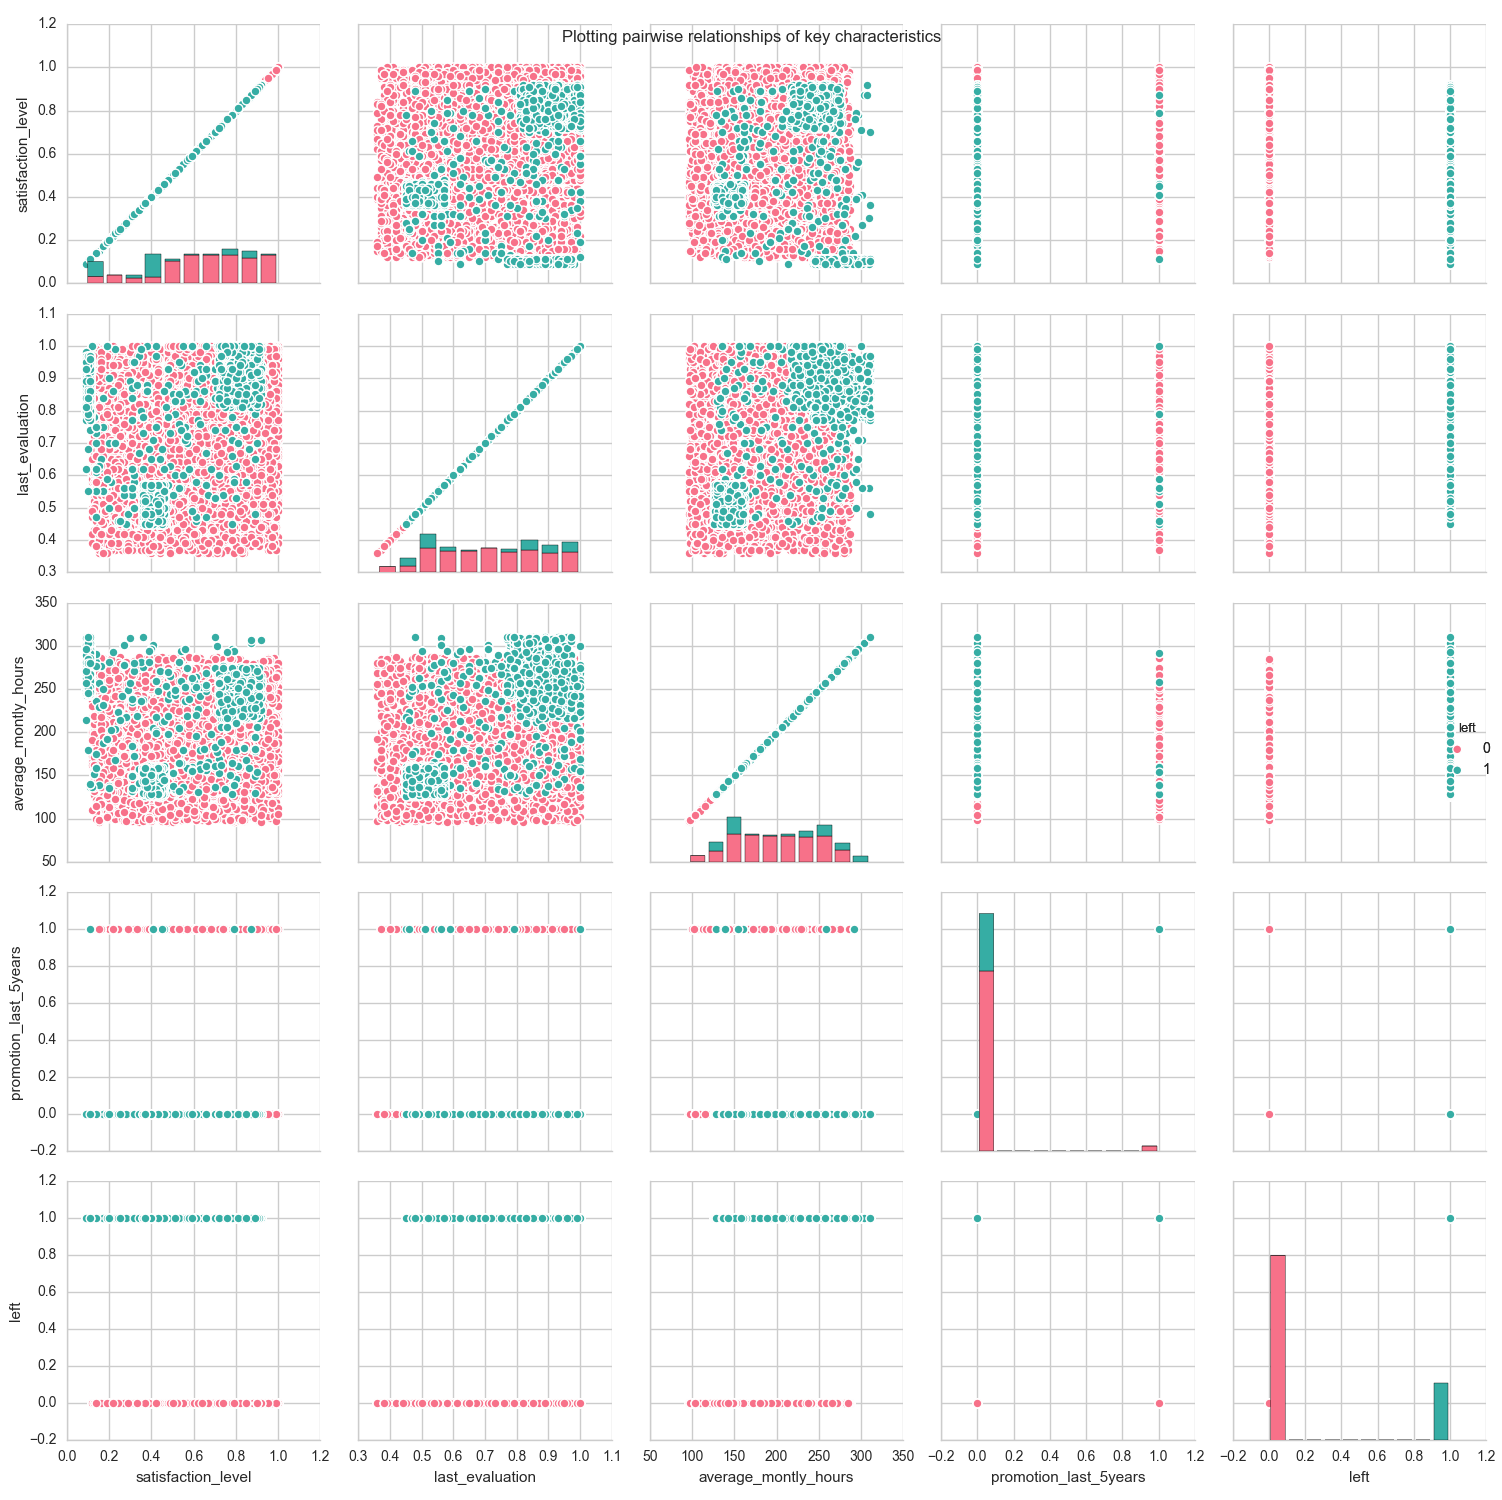
\includegraphics{images/pairwise_plot.png}}}
\end{figure}
\flushleft
Using the \href{https://www.kaggle.com/ludobenistant/hr-analytics}{Human Resources Analytics dataset} from Kaggle, I conducted a preliminary analysis on characteristics that affect employees to leave rather than stay. I began my exploring the data by visualizing the data with a heatmap of the correlations between all the variables, and found that  work accidents and number of projects are weakly correlated with leaving the company. \
\flushleft 
Thus, I did a pairwise plot with the key characteristics, satisfaction levels, average monthly hours, number of projects, last evaluations, promotion over the last 5 years and employee leaving or staying. From Figure 1, we can observe high correlations wherever clusters exist and conclude with the following:
\begin{itemize}
  \item Employees that left the organisation have lower satisfaction levels, works high number of hours even though their last evaluations were pretty high.
  \item Most of the employees that left rarely had a promotion over the last five years.
\end{itemize}
 
\newpage
\noindent\textbf{Problem 2}\\
\flushleft In Monteforte’s and Moretti’s recent paper on “Real-Time Forecasts of Inflation: The Role of Financial Variables”\textsuperscript{1} (2013), they attempt to augment inflation forecasting with daily data from financial markets and found that the addition of daily variable reduces forecasting errors, when compared to models that only factor in monthly variables. The issue pointed out by Monteforte and Moretti is that monthly indicators do not capture important information within the month. Thus, they attempt to mitigate the gap by including daily data from financial indicators such as movements in the yield curve or interest rate spread, and combine it with the monthly core inflation index with daily prices of commodities and financial assets. \\
\flushleft
While their paper is already an improvement in forecasting inflation with more real-time data, the advent of the internet and crowdsourcing platforms enable researchers to collect daily prices of commodities with human computation projects. These days, it is uncommon for individuals to log their groceries expenditure to track their expenses and monitor their dietary intake. Individuals can be encouraged to make it a habit to contribute such information on an open source website. Besides, being a platform to log their groceries expenditure, social elements could be incorporated into the site, where people create sub-threads about tips on eating clean and reducing costs of doing so. Such data can then be collected and replace daily proxies of inflation per month. These newly available data through human computation projects could be an additional input to the Mixed Data Sampling Regression Models (MIDAS), as implemented in Monteforte’s and Moretti’s paper, and would be likely to further reduce errors in forecasting inflation. \\
\flushleft
\textbf{References}

[1] Monteforte, Libero, and Gianluca Moretti. "Real‐Time Forecasts of Inflation: The Role of Financial Variables." Journal of Forecasting 32, no. 1 (2013): 51-61.
\end{document}
